\documentclass[12pt]{article}

% PACKAGES
\usepackage[ngerman]{babel}
\usepackage{lmodern} % Schriftart
\usepackage{bookmark} % Für PDF Lesezeichen
\usepackage{caption} % Für \caption*{}
\usepackage{siunitx} % SI-Einheiten
\usepackage{mathtools} % Verbessertes "amsmath" (https://de.overleaf.com/learn/latex/Articles%2FMathtools_-_for_beautiful_math)
\usepackage{xcolor}   % Farbiger Text (https://www.overleaf.com/learn/latex/Using_colours_in_LaTeX)
\usepackage{geometry} % Zur Einstellung des Layouts
\usepackage{titlesec} % Einteilung des Inhalts (https://de.overleaf.com/learn/latex/Sections_and_chapters)
\usepackage{fancyhdr} % Für Kopf-/ und Fußzeilen (https://www.overleaf.com/learn/latex/Headers_and_footers)
\usepackage{parskip} % Änderung von Absätzen und Absatzeinzügen
\usepackage{biblatex} % Verweise und Referenzen
\usepackage{float} % Benötogt für Figuren und Tabellen
\usepackage{graphicx} % Platzhalter Bilder
\usepackage{booktabs} % Tabellen
\usepackage{csquotes} % Recommended package for biblatex
\usepackage{hyphenat}
\usepackage{listings} % for typesetting code
\usepackage{graphicx}
\usepackage{caption}
\usepackage{subcaption}
% SETUP 
\setlength{\headheight}{15.059pt} % Set headheight to at least 14.5pt
\addtolength{\topmargin}{-2.5pt} % Make topmargin smaller to compensate
\sisetup{
  output-decimal-marker={,},
  per-mode=fraction,
  fraction-function=\tfrac,
  separate-uncertainty=true
}

\addbibresource{Ressourcen/V51.bib}
\geometry{ %A4
  a4paper,
  total = {170mm,240mm},
  left = 20mm,
  top = 30mm
}
\pagestyle{fancy}
\captionsetup[figure]{
    justification=centering, % Centered captions
    labelsep=colon, % Separate label and caption with a period
    singlelinecheck=false, % Always center even if the caption is short
    labelfont=bf % Bold captions
}
% COMMANDS
\newcommand{\uproman}[1]{\uppercase\expandafter{\romannumeral#1}} % Römische Zahlen

\sisetup{
  per-mode=fraction,
  fraction-function=\tfrac,
  separate-uncertainty=true,
  output-decimal-marker={,}
}
% DOC
\begin{document}

% HEADER
\begin{titlepage}
  \centering
  \vspace*{1cm}
  
\includegraphics[width=0.5\textwidth]{Ressourcen/tud_logo_schwarz(RGB)}\\
  \vspace*{0.25cm}
  \large\textmd{Fakultät Physik} \\
  \vspace*{6cm}
  \huge \bfseries FP-2024 - Versuch V51\\
  \vspace*{0.25cm}
  \large Operationsverstärker\\
  \vspace*{0.25cm}
  \large\textmd{\href{mailto:jan.oppoli@tu-dortmund.de}{Jan Oppoli}} \\
  \vfill
  \small\textmd{Versuch durchgeführt am 27. Mai 2024}\\
  \small\textmd{Abgabe erstellt am 21. Juni 2024}
\end{titlepage}
\tableofcontents 
\newpage

\section{Zielsetzung}\label{sec:zielsetzung}
Ziel dieses Versuchs ist es, die Funktionsweise des Operationsverstärkers zu erschließen, indem verschiedene Schaltkreise, die diesen enthalten, untersucht werden. Infolge dessen werden ebenfalls die Kenngrößen sowohl der Schaltungen als auch des Verstärkers bestimmt.

\section{Theorie}\label{sec:theorie}
Im Allgemeinen müssen für das vorliegende Experiment zwei Bereiche genauer beleuchtet werden: das Prinzip eines Operationsverstärkers sowie grundsätzliche Gesetze und das Verhalten von elektrischen Schaltungen.

\subsection{Operationsverstärker}
Ein Operationsverstärker, oft als Op-Amp bezeichnet, ist ein integrierter Schaltkreis, der als Spannungsverstärker fungiert. Er hat zwei Eingänge und einen Ausgang. Die beiden Eingänge werden als invertierender Eingang (\( U_- \)) und nicht-invertierender Eingang (\( U_+ \)) bezeichnet.

\subsubsection{Grundprinzipien}
\begin{itemize}
    \item \textbf{Invertierender Eingang (\( U_- \))}: Ein Signal, das an diesen Eingang angelegt wird, wird am Ausgang des Verstärkers umgekehrt (invertiert).
    \item \textbf{Nicht-invertierender Eingang (\( U_+ \))}: Ein Signal, das an diesen Eingang angelegt wird, wird am Ausgang verstärkt, ohne die Polarität zu ändern.
\end{itemize}

\subsubsection{Grundgleichung des Operationsverstärkers}
Die Ausgangsspannung eines idealen Operationsverstärkers, abhängend von den zwei Eingangsspannungen lässt sich durch die folgende Gleichung beschreiben:
\[
U_{\text{out}} = A_{\text{ol}} (U_+ - U_-)
\]
wobei \( A_{\text{ol}} \) die Leerlaufverstärkung des Operationsverstärkers ist, die in idealen Fällen sehr hoch ist.

\subsubsection{Eigenschaften von Operationsverstärkern}
Ideale Operationsverstärker besitzen eine unendliche Verstärkung (\( A_{\text{ol}} \)), was bedeutet, dass selbst ein kleiner Unterschied zwischen \( V_+ \) und \( V_- \) eine große Ausgangsspannung erzeugt. In der Realität ist die Verstärkung jedoch endlich, wenn auch sehr hoch, was zu geringfügigen Abweichungen führt. 

Ein idealer Operationsverstärker hat einen unendlichen Eingangswiderstand, sodass kein Strom in die Eingänge fließt. Im Gegensatz dazu haben reale Operationsverstärker einen sehr hohen, aber endlichen Eingangswiderstand, was minimalen Stromfluss ermöglicht. Der Ausgangswiderstand eines idealen Operationsverstärkers ist null, wodurch der Ausgang beliebig viel Strom liefern kann, ohne dass die Ausgangsspannung abfällt. In der Praxis weisen reale Operationsverstärker einen kleinen, aber nicht vernachlässigbaren Ausgangswiderstand auf.

Weiterhin besitzt ein idealer Operationsverstärker eine unendliche Bandbreite, was bedeutet, dass er Signale aller Frequenzen verstärken kann. Reale Operationsverstärker haben hingegen eine begrenzte Bandbreite, was die Verstärkung Signale bestimmter Frequenzen einschränkt. Schließlich weist ein idealer Operationsverstärker keine Offset-Spannung auf, sodass \( V_{\text{out}} \) gleich null ist, wenn \( V_+ = V_- \). In der Realität existiert jedoch eine geringe Offset-Spannung, die durch Kalibrierung minimiert werden kann.


\subsubsection{Anwendungen von Operationsverstärkern}
Operationsverstärker können in einer Vielzahl von Anwendungen eingesetzt werden, darunter:
\begin{itemize}
    \item \textbf{Verstärker}: Wie in invertierenden und nicht-invertierenden Verstärkerschaltungen.
    \item \textbf{Filter}: Zur Frequenzselektion und Signalbearbeitung.
    \item \textbf{Integrator und Differentiator}: Zur Durchführung mathematischer Operationen auf Signale.
    \item \textbf{Schmitt-Trigger}: Zur Umwandlung eines analogen Signals in ein digitales Signal mit Hysterese.
\end{itemize}
\subsection{Gesetze elektrischer Schaltkreise}
Die wichtigsten zwei Formeln zur Beschreibung des Verhaltens von Schaltungen sind die Kirchoffschen Gesetze\cite{kirchhoff1845durchgang}.
Der Knotenpunktsatz für einen Knoten mit $n$ ein- und ausgehenden Strömen
\begin{align}
  \sum_{k=1}^n I_k=0
\end{align}
besagt, dass die Summe der zufließenden Ströme gleich der Summe der abfließenden Ströme ist.\\
Der Maschensatz
\begin{align}
  \sum_{k=1}^nU_k=0\text{,}
\end{align}
mit Teilspannungen $U_k$ einer Masche innerhalb eines elektrischen Netzwerkes besagt wiederum, dass die Summe aller Teilspannungen sich zu Null addiert. Die Spannungen welche der beliebig gewählten Umlaufrichtung entgegenwirken müssen mit einem negativen Vorzeichen versehen werden.
\section{Aufbau}
Im wesentlichen besteht der Versuchsaufbau aus einer Steckplatine wie in \autoref{fig:1} abgebildet, einem Signalgenerator sowie einem Oszilloskop. Die zu untersuchenden Schaltkreise werden mithilfe der einzelnen Komponenten und Verbindungskabeln konstruiert und die gemessenen Spannungssignale anschließend auf dem Bildschirm grafisch ausgegeben.
\begin{figure}[H]
  \centering
  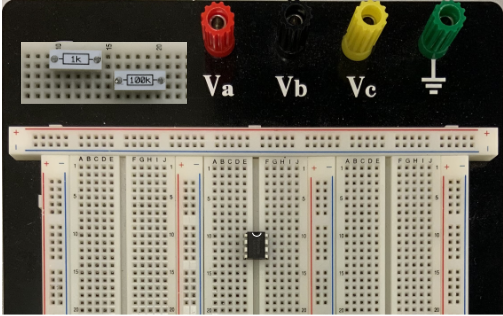
\includegraphics[scale=0.5]{Ressourcen/breadbord.png}
  \caption{Die für den Versuch verwendete Steckplatine\cite{anleitung}.}\label{fig:1}
\end{figure}
Unter Kombination der zuvor genannten Komponenten werden fünf verscheidene Schaltkreise aufgebaut, welche im Anschließenden erläutert werden:
\subsubsection{Invertierender Verstärker}

Ein invertierender Verstärker wie er in \autoref{fig:2} zu sehen ist, verstärkt die Eingangsspannung und invertiert sie um 180 Grad.
\begin{figure}[H]
  \centering
  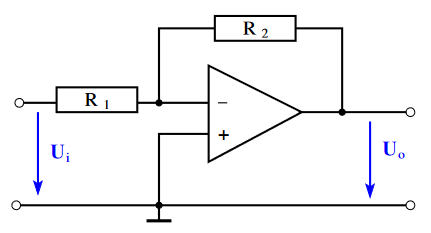
\includegraphics[scale=0.8]{Ressourcen/invamp.png}
  \caption{Schaltplan eines invertierenden Verstärkers\cite{anleitung}.}\label{fig:2}
\end{figure}
Er besteht aus einem Operationsverstärker (Op-Amp), einem Eingangswiderstand \( R_1 \) und einem Rückkopplungswiderstand \( R_2 \).

Die Ausgangsspannung \( U_o \) ist durch die Verstärkung

\begin{equation}
    V = - \frac{R_2}{R_1}
\end{equation}
bestimmt, woraus die Formel

\begin{equation}
    U_o = - V U_i = - \left( \frac{R_2}{R_1} \right) U_i
\end{equation}
folgt.
\subsection{Integrator}
Ein invertierender Integrator, in \autoref{fig:3} zu sehen, wandelt die Eingangsspannung in eine Ausgangsspannung um, die das Integral der Eingangsspannung darstellt.
\begin{figure}[H]
  \centering
  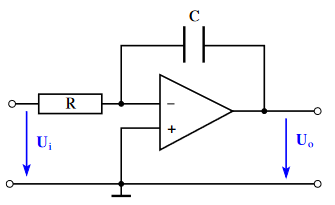
\includegraphics[scale=0.8]{Ressourcen/integrator.png}
  \caption{Schaltplan eines Integrators\cite{anleitung}.}\label{fig:3}
\end{figure}
Er besteht aus einem Operationsverstärker (Op-Amp), einem Eingangswiderstand \( R \) und einem Rückkopplungskondensator \( C \).

Die Ausgangsspannung \( U_o \) ist gemäß der Kirchhoffschen Gesetze durch die folgende Differentialgleichung bestimmt:
\begin{equation}
  \frac{dU_o(t)}{dt} = -\frac{1}{RC} U_i(t)
\end{equation}


Der Zusammenhang zwischen Ein- und Ausgangsspannung wird durch die Beziehung

\begin{equation}
  U_o(t) = -\frac{1}{RC} \int_0^t U_i(\tau) \, d\tau\label{eqn:int}
\end{equation}

beschrieben.
\subsection{Differenzierer}
Ein Differenzierer wandelt die Eingangsspannung wie in \autoref{fig:4} abgebildet in eine Ausgangsspannung um, die die Ableitung der Eingangsspannung darstellt.
\begin{figure}[H]
  \centering
  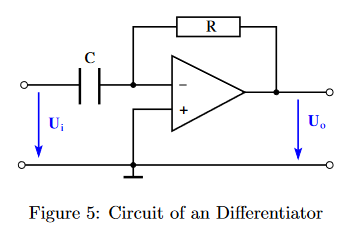
\includegraphics[scale=0.8]{Ressourcen/differentiator.png}
  \caption{Schaltplan eines Differenzierers\cite{anleitung}.}\label{fig:4}
\end{figure}
Er besteht aus einem Operationsverstärker (Op-Amp), einem Eingangskondensator \( C \) und einem Rückkopplungswiderstand \( R \).

Die Ausgangsspannung \( U_o \) ist entsprechend der Kirchhoffschen Gesetze durch die folgende Differentialgleichung bestimmt:

\begin{equation}
    U_o(t) = -RC \frac{dU_i(t)}{dt}.\label{eqn:diff}
\end{equation}
\subsection{Schmitt-Trigger}
Ein Schmitt-Trigger ist eine elektronische Schaltung, die als Komparator mit Hysterese funktioniert und zur Signalverarbeitung verwendet wird. Zu sehen ist dieser in \autoref{fig:5}
\begin{figure}[H]
  \centering
  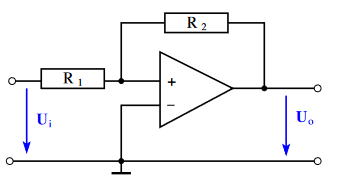
\includegraphics[scale=0.8]{Ressourcen/schmitt.png}
  \caption{Schaltplan eines Schmitt-Triggers\cite{anleitung}.}\label{fig:5}
\end{figure}
Er besteht aus einem Operationsverstärker (Op-Amp), einem Eingangswiderstand \( R_1 \) und einem Rückkopplungswiderstand \( R_2 \).

Die Ausgangsspannung \( U_o \) schaltet zwischen zwei definierten Spannungspegeln, abhängig von der Eingangsspannung \( U_i \). Der Schaltvorgang erfolgt bei den Schwellwerten \( U_{TH+} \) und \( U_{TH-} \), die durch die Widerstände bestimmt werden:

\begin{equation}
    U_{TH+} = \frac{R_2}{R_1 + R_2} V_{out+}\label{eqn:schwell}
\end{equation}

\begin{equation}
    U_{TH-} = \frac{R_2}{R_1 + R_2} V_{out-}
\end{equation}

Hierbei sind \( V_{out+} \) und \( V_{out-} \) die positiven und negativen Sättigungsspannungen des Operationsverstärkers.
\subsection{Generator}
Ein Signalgenerator kann durch die Verbindung eines Schmitt-Triggers mit einem invertierenden Integrator realisiert werden. Wie in \autoref{fig:6} dargestellt, beginnt dieses System spontan zu schwingen.
\begin{figure}[H]
  \centering
  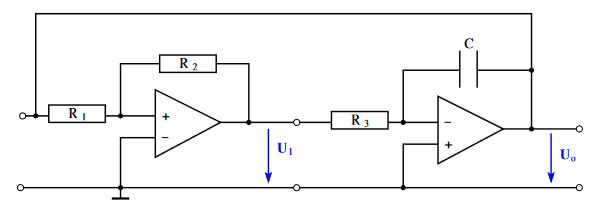
\includegraphics[scale=0.8]{Ressourcen/generator.png}
  \caption{Schaltplan eines Signalgenerators\cite{anleitung}.}\label{fig:6}
\end{figure}
Der Schmitt-Trigger erzeugt eine konstante Ausgangsspannung, die zwischen zwei definierten Spannungspegeln wechselt. Diese Spannung wird dem Eingang des Integrators zugeführt. Der Integrator wandelt die konstante Spannung in eine lineare Rampenspannung um, die die Ausgangsspannung \( U_1 \) darstellt. 

Wenn die Ausgangsspannung \( U_1 \) des Integrators einen der Schwellenwerte des Schmitt-Triggers erreicht, schaltet der Schmitt-Trigger seinen Ausgangszustand um. Dadurch ändert sich die Vorzeichen der Spannung, die dem Integrator zugeführt wird, und die Richtung der Rampenfunktion kehrt sich um. Dies führt zu einer kontinuierlichen Dreieckspannung am Ausgang des Integrators.

Die Frequenz der Dreieckspannung \( \nu_\text{Dreieck} \) kann durch die folgenden Parameter bestimmt werden:

\begin{equation}
    \nu_\text{Dreieck} = \frac{R_2}{4 C R_1 R_3}
    \label{eqn:fdrei}
\end{equation}

Die Amplitude der Dreiecksspannung \( A \) wird durch das Verhältnis der Widerstände des Schmitt-Triggers und die maximale Ausgangsspannung \( U_\text{max} \) des Schmitt-Triggers bestimmt:

\begin{equation}
    A = U_\text{max} \frac{R_1}{R_2}
    \label{eqn:amp2}
\end{equation}

Dieses System ermöglicht die Erzeugung einer stabilen Dreieckspannung, deren Frequenz und Amplitude durch die Wahl der Widerstände und des Kondensators bestimmt werden können.
\subsection{Generator mit variierender Amplitude}
Ein Generator mit variierender Amplitude besteht aus zwei Integratoren und einem Invertierer, wodurch eine gedämpfte Oszillation erzeugt werden kann. Der Aufbau des Systems ist in \autoref{fig:7} dargestellt.
\begin{figure}[H]
  \centering
  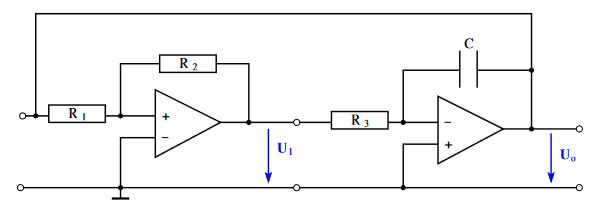
\includegraphics[scale=0.8]{Ressourcen/generator.png}
  \caption{Schaltplan eines Signalgenerators mit variierender Amplitude\cite{anleitung}.}\label{fig:7}
\end{figure}

Die gedämpfte Oszillation wird durch die Differentialgleichung

\begin{equation*}
    \frac{\mathrm{d}^2 U_A}{\mathrm{d}t^2} - \frac{\eta}{10RC} \frac{\mathrm{d}U_A}{\mathrm{d}t} + \frac{1}{R^2 C^2} U_A = 0
\end{equation*}

beschrieben, wobei \( \eta \) die Dämpfungskonstante darstellt.

Die Lösung dieser Gleichung ist gegeben durch

\begin{equation}
    U_A(t) = U_0 \cdot \exp\left( -\frac{t}{\tau} \right) \cdot \sin\left( 2\pi \frac{t}{T} \right)
    \label{eqn:dgllsg}
\end{equation}

Dabei sind die Abklingdauer \( \tau \) und die Schwingungsdauer \( T \) als

\begin{equation}
    \tau = \frac{20RC}{\eta}
    \label{eqn:tau}
\end{equation}
und 
\begin{equation}
    T = 2\pi RC
\end{equation}
definiert.
\section{Durchführung}\label{sec:durchfuehrung}
\subsection{Invertierender Verstärker}
Nachdem die korrekte Schaltung aufgebaut wurde, wurden für \( R_1 = \SI{1}{\kilo\ohm} \) und \( R_2 = \SI{100}{\kilo\ohm} \) die frequenzabhängigen Amplituden \( U_0 \) gemessen. Die Ergebnisse wurden in einem doppelt-logarithmischen Diagramm (Bode-Diagramm) dargestellt.

\subsection{Integrator}
Für den Integrator wurden \( R = \SI{10}{\kilo\ohm} \) und \( C = \SI{100}{\nano\farad} \) verwendet. Die Frequenzabhängigkeit der Eingangs- und Ausgangsspannungen wurde gemessen und die Ausgangssignale für anfäng-liche Dreieck- und Rechteck-Eingangssignale angezeigt.

\subsection{Differentiator}
Die Schaltung des Differentiators wurde mit \( R = \SI{100}{\kilo\ohm} \) und \( C = \SI{22}{\nano\farad} \) aufgebaut. Die Messungen wurden analog zur Analyse des Integrators durchgeführt.

\subsection{Schmitt-Trigger}
Der Schmitt-Trigger wurde mit \( R_1 = \SI{10}{\kilo\ohm} \) und \( R_2 = \SI{100}{\kilo\ohm} \) aufgebaut. Die Amplitude wurde in Schritten von wenigen Millivolt erhöht und der Kipppunkt mit einem Oszilloskop bestimmt. Mehrere Messpunkte wurden gemittelt, um den genauen Kipppunkt zu ermitteln.

\subsection{Generator}
Die Generatorschaltung wurde mit den Komponenten \( R_1 = \SI{10}{\kilo\ohm} \), \( R_2 = \SI{100}{\kilo\ohm} \), \( R_3 = \SI{1}{\kilo\ohm} \) und \( C = \SI{1}{\micro\farad} \) aufgebaut. Mit dem Oszilloskop wurden die Signale \( U_1 \) und \( U_0 \) gemessen und die Frequenz sowie die Amplituden aufgenommen.

\subsection{Generator mit variierender Amplitude}\label{subsec:vargen}
Die Generatorschaltung wurde mit den Komponenten \( R = \SI{10}{\kilo\ohm} \), \( R = \SI{1}{\kilo\ohm} \), \( 10R \), und \( C = \SI{22}{\nano\farad} \) bzw. \( C = \SI{100}{\nano\farad} \) aufgebaut. Die Periodendauer \( T \) und die Abklingdauer \( \tau \) wurden gemessen. Für \( \eta < 0 \) wurde eine gedämpfte Oszillation aufgezeichnet, wobei die Dämpfung der Oszillation gemessen und in einem halblogarithmischen Diagramm dargestellt wurde. Für \( \eta > 0 \) wurde die Periodendauer der Oszillation gemessen.

\section{Auswertung}\label{sec:auswertung}
Zunächst eine kurze Erläuterung des verwendeten Fehlerrechnungsformalismus.
\subsection{Fehler und Messunsicherheiten}\label{subsec:fehler-und-messunsicherheiten}
Jegliche Fehlerfortpflanzungen und Berechnungen mit Messunsicherheiten finden durch das Python-Package Uncertainties\cite{uncertainties} statt.
Somit werden einmal alle bekannten Variablen einmal mit einer speziellen Funktion aus Uncertainties festgelegt.
Bei allen nachfolgenden Berechnungen erfolgen die benötigten Fortpflanzungen durch Uncertainties automatisch.
Die Formel für die Fehlerfortpflanzung ist
\begin{align}
  \Delta y=\sum_{i=1}^n\left|\frac{\delta f\left(x_1, \ldots, x_n\right)}{\delta x_i}\right| \Delta x_i.\text{.}\label{gauss}
\end{align}
und die Formel für den Mittelwert/ das arithmetische Mittel ist
\begin{align}
  \bar{x}=\frac{1}{n}\sum_{i=1}^n x_i\label{mittel}
\end{align}
Wie die Ableitungen bestimmt werden ist in der \href{https://readthedocs.org/projects/uncertainties-python-package/downloads/pdf/latest/}{Technischen Dokumentation} selbst nachzulesen.
\subsection{Invertierender Verstärker}
Die aufgenmomenen Messwerte der Ein- und Ausgangsspannungen $U_\text{i}$ und $U_0$ sowie der Phasenverschiebung $\phi$ in Abhängigkeit der Frequenz $f$ inklusive der verwendeten Widerstände sind in \autoref{tab:1} zu sehen.
\begin{table}[H]
  \centering
  \caption{Messwerte des Invertierenden Linearverstärkers mit $R_1=1\unit{\kilo\ohm}$ und $R_2=100\unit{\kilo\ohm}$}
  \begin{tabular}{r | c c c}
  \toprule
   $f\mathbin{/}\unit{\hertz}$ &  $U_0\mathbin{/}\unit{\volt}$&  $U_{\text{i}}\mathbin{/}\unit{\volt}$ & $\phi\mathbin{/}$ rad\\
  \midrule
  5&23.52&0.24&3.13\\
  30&23.27&0.264&3.15\\
  50&23.4&0.252&3.14\\
  100&23.16&0.264&3.13\\
  250&23.63&0.24&3.12\\
  500&23.27&0.252&3.14\\
  1000&23.52&0.264&3.06\\
  2000&22.92&0.24&2.96\\
  4000&21.96&0.264&2.73\\
  7500&18.0&0.252&2.33\\
  15000&10.68&0.24&1.82\\
  30000&6.24&0.288&1.7\\
  60000&3.36&0.276&1.6\\
  120000&2.04&0.288&1.44\\
  240000&1.56&0.264&1.21\\
  \bottomrule
  \end{tabular}
  \label{tab:1}
\end{table}

Die Messdaten wurden analysiert, um das Verhältnis der Ausgangsspannung zur Eingangsspannung in Abhängigkeit der Frequenz zu untersuchen. Das Verhältnis $U_0/U_i$ wurde für jede Frequenz berechnet und in einem doppelt-logarithmischen Diagramm dargestellt. Zusätzlich wurde mithilfe der Python Bibliothek SciPy eine Ausgleichsgerade der Form
\begin{align}
  U_\text{fit}(f)=m\cdot \ln{f}+b
\end{align}
für die höheren Frequenzen berechnet sowie der Mittelwert und die Standardabweichung des Spannungsverhältnisses für die niedrigeren Frequenzen ermittelt\cite{scipy}. Die Unsicherheiten des Mittelwerts wurden als markierter Bereich um die Linie herum dargestellt. Die entsprechenden Diagramme sind in \autoref{fig:invamp_plot} zu sehen.

\begin{figure}[H]
  \centering
  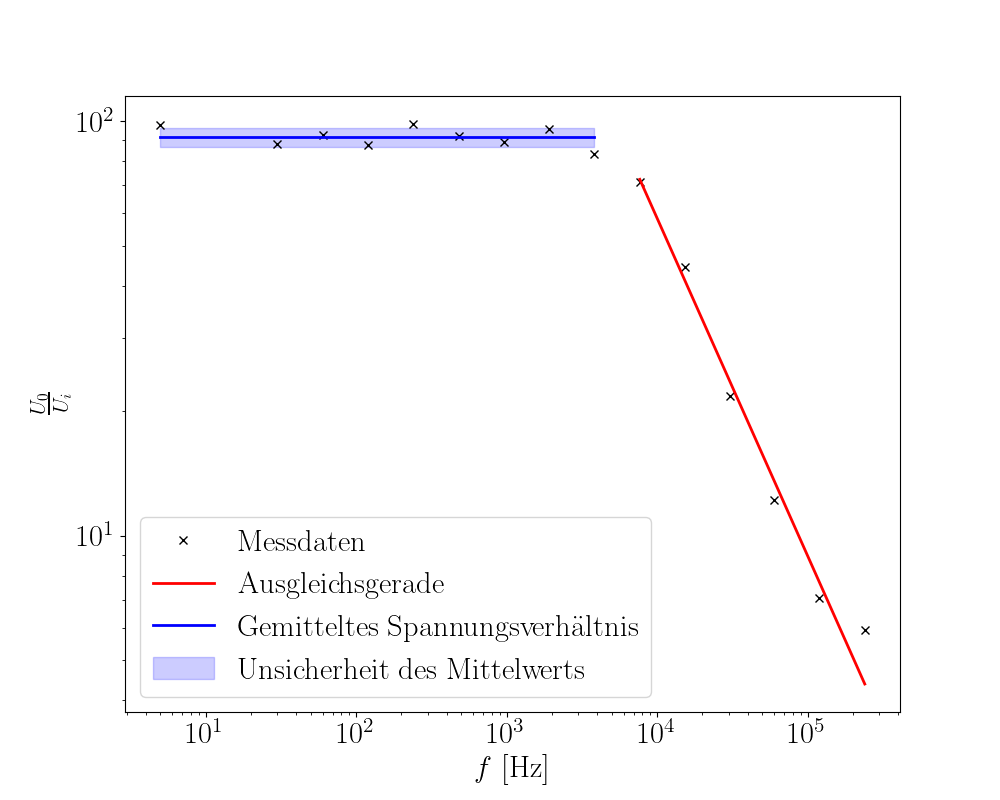
\includegraphics[width=0.8\textwidth]{../Ressourcen/invamp_plot.png}
  \caption{Darstellung des Verhältnisses $U_0/U_i$ in Abhängigkeit der Frequenz $f$ inklusive Fit.}
  \label{fig:invamp_plot}
\end{figure}

Die Parameter der Ausgleichsgeraden sind in \autoref{tab:fitparams} aufgelistet.

\begin{table}[H]
  \centering
  \caption{Fit-Parameter der Ausgleichsgeraden}
  \begin{tabular}{c c}
  \toprule
  Parameter & Wert \\
  \midrule
  Steigung $m$ & $\SI{-0.81(0.04)}{\second}$ \\
  Achsenabschnitt $b$ & $11.57\pm0.41$ \\
  \bottomrule
  \end{tabular}
  \label{tab:fitparams}
\end{table}

Der Mittelwert des Spannungsverhältnisses, die Leerlaufverstärkung für die niedrigeren Frequenzen beträgt
\begin{align}
  V_\text{invamp} = \overline{\frac{U_0}{U_\text{i}}}=91.70\pm4.82
\end{align}
und somit ergibt sich für die Grenzfrequenz bei welcher die Intensität um einen Faktor $\frac{1}{\sqrt{2}}$ gefallen ist
\begin{align}
  f_\text{grenz}=\SI{9538.98(962.41)}{\hertz}\text{,}
\end{align}
wobei der Wert mittels Interpolation gefunden wurde.
Letzendlich lässt sich das Bandbreitenprodukt als
\begin{equation*}
  V_\text{invamp}\cdot f_{\text{grenz}}=\SI{8.74(0.95)e5}{\hertz}
\end{equation*}
berechnen. Die theoretische Leerlaufverstärkung beträgt
\begin{align}
  V_\text{theorie} = 100.
\end{align}
\\
In Absprache mit der Versuchsleitung wurde aufgrund von fehlerhafter Hardware und zeitlichen Beschränkungen auf die ergänzenden Messungen mit zusätzlichen Widerstandsverhältnissen $\frac{R_1}{R_2}$ verzichtet.
\subsection{Integrator}
Die Aufgenommenen Messwerte des Integrators sind in \autoref{tab:2} angeführt und anschließend in \autoref{fig:8} visuell dargestellt.
\begin{table}[H]
  \centering
  \caption{Messwerte des Invertierenden Linearverstärkers mit $R=10\unit{\kilo\ohm}$ und $C=100\unit{\nano\farad}$}
  \begin{tabular}{r | c c}
  \toprule
   $f\mathbin{/}\unit{\hertz}$ &  $U_0\mathbin{/}\unit{\volt}$&  $U_{\text{i}}\mathbin{/}\unit{\volt}$ \\
  \midrule
  40& 10.6&39.1\\
  50& 10.6&31.8\\
  60& 10.6&26.3\\
  70& 10.6&23.6\\
  80& 10.6&20.7\\
  90& 10.6&18.3\\
  100& 10.6&17.1\\
  150& 10.6&12.3\\
  170& 10.6&10.6\\
  200& 10.6&9.4\\
  250& 10.6&7.7\\
  500& 10.6&3.3\\
  \bottomrule
  \end{tabular}
  \label{tab:2}
\end{table}
Es ist zu erkennen, dass das Amplitudenverhältnis im doppellogarithmischen Diagramm linear zu fallen Scheint, was im Vergleich mit \autoref{eqn:int} Sinn ergibt, da aus Integration einer Periodischen Sinusfunktion mit der Frequenz $f$ unter anderem der entscheidende Vorfaktor $\frac{1}{f}$ entsteht.
Dieser spiegelt sich dann als linearer Abfall wieder.
\begin{figure}[H]
  \centering
  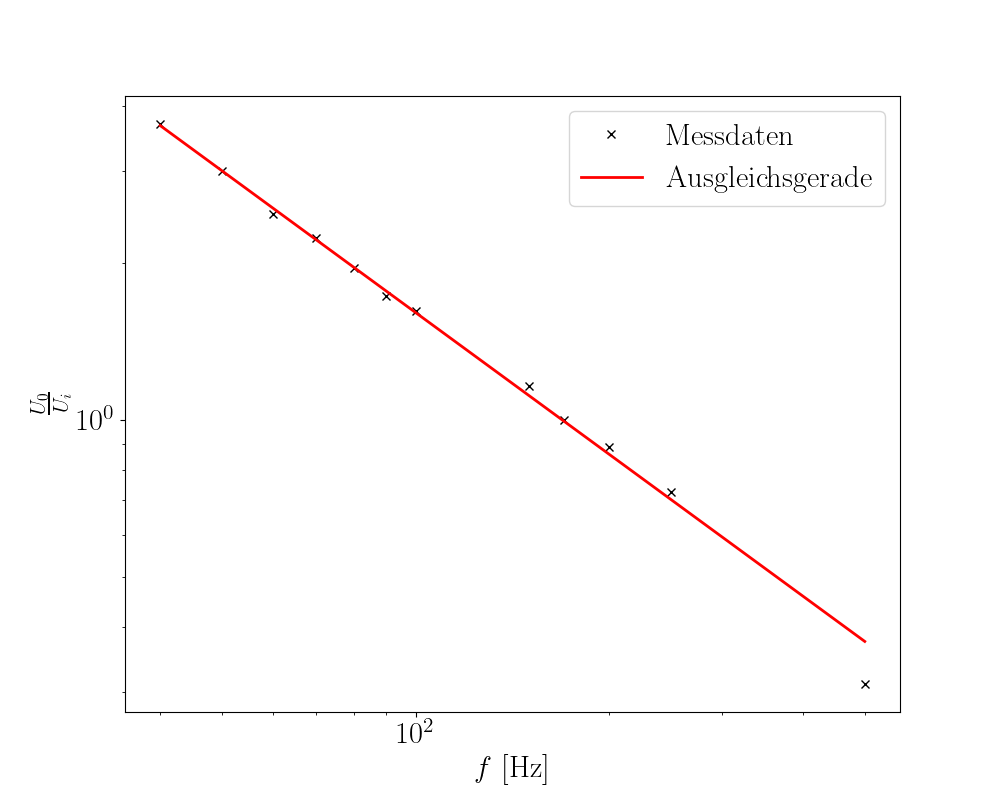
\includegraphics[width=0.8\textwidth]{../Ressourcen/integrator_plot.png}
  \caption{Darstellung des Verhältnisses $U_0/U_i$ in Abhängigkeit der Frequenz $f$ für den Integrator, inklusive einer Ausgleichsgerade.}
  \label{fig:8}
\end{figure}
Nach erneutem Fit an die Messwerte ergeben sich die Parameter, welche in \autoref{tab:fitparams2} zu sehen sind.
\begin{table}[H]
  \centering
  \caption{Fit-Parameter der Ausgleichsgeraden des Integrators}
  \begin{tabular}{c c}
  \toprule
  Parameter & Wert \\
  \midrule
  Steigung $m$ & $\SI{-0.902(0.013)}{\second}$ \\
  Achsenabschnitt $b$ & $4.62\pm0.05$ \\
  \bottomrule
  \end{tabular}
  \label{tab:fitparams2}
\end{table}
Als ideale Zeitkonstante des Aufbaus folgt
\begin{align}
  \tau = R\cdot C = \SI{1}{\milli\second}\text{,}
\end{align}
womit sich die Ideal erwarteten Funktionsparameter
\begin{align}
  m_\text{theorie} &= \SI{-1}{\second}\\
  b_\text{theorie} &=\ln\left(\frac{1}{RC}\right) = 6.91
\end{align}
berechnen lassen.
\subsection{Differentiator}
Die Aufgenommenen Messwerte des Differentiators sind in \autoref{tab:3} angeführt und anschließend in \autoref{fig:9} visuell dargestellt.
\begin{table}[H]
  \centering
  \caption{Messwerte des Differentiators mit $R=100\unit{\kilo\ohm}$ und $C=22\unit{\nano\farad}$}
  \begin{tabular}{r | c c}
  \toprule
   $f\mathbin{/}\unit{\hertz}$ &  $U_0\mathbin{/}\unit{\volt}$ &  $U_{\text{i}}\mathbin{/}\unit{\volt}$ \\
  \midrule
  40 & 6.0 & 10.6 \\
  50 & 7.6 & 10.6 \\
  60 & 9.0 & 10.6 \\
  70 & 10.5 & 10.6 \\
  80 & 12.0 & 10.6 \\
  90 & 13.1 & 10.6 \\
  100 & 14.3 & 10.6 \\
  150 & 21.0 & 10.6 \\
  200 & 27.1 & 10.6 \\
  250 & 33.0 & 10.6 \\
  500 & 66.0 & 10.6 \\
  \bottomrule
  \end{tabular}
  \label{tab:3}
\end{table}
Es ist zu erkennen, dass das Amplitudenverhältnis im doppellogarithmischen Diagramm linear zu steigen scheint, was im Vergleich mit \autoref{eqn:diff} Sinn ergibt, da aus Differentiation einer periodischen Sinusfunktion mit der Frequenz $f$ unter anderem der entscheidende Vorfaktor $f$ entsteht.
Dieser spiegelt sich dann als linearer Anstieg wieder.
\begin{figure}[H]
  \centering
  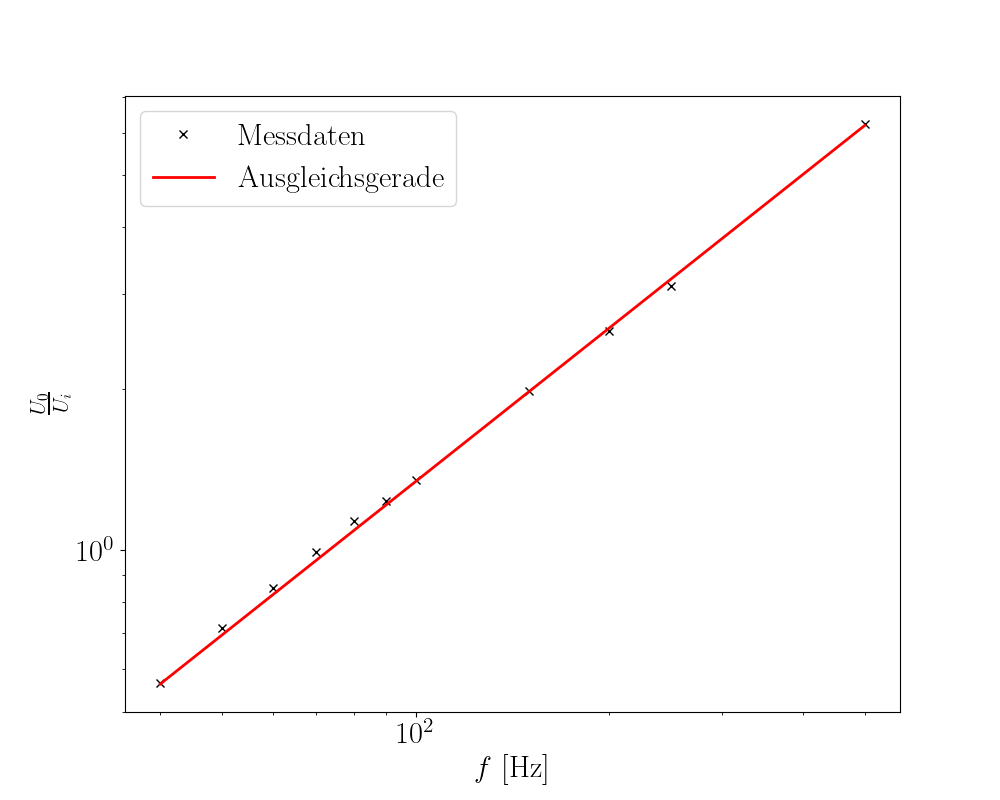
\includegraphics[width=0.8\textwidth]{../Ressourcen/differentiator_plot.png}
  \caption{Darstellung des Verhältnisses $U_0/U_i$ in Abhängigkeit der Frequenz $f$ für den Differentiator, inklusive einer Ausgleichsgerade.}
  \label{fig:9}
\end{figure}
Nach erneutem Fit an die Messwerte ergeben sich die Parameter, welche in \autoref{tab:fitparams3} zu sehen sind.
\begin{table}[H]
  \centering
  \caption{Fit-Parameter der Ausgleichsgeraden des Differentiators}
  \begin{tabular}{c c}
  \toprule
  Parameter & Wert \\
  \midrule
  Steigung $m$ & $\SI{0.949(0.008)}{\second}$ \\
  Achsenabschnitt $b$ & $-4.07\pm0.05$ \\
  \bottomrule
  \end{tabular}
  \label{tab:fitparams3}
\end{table}
Als ideale Zeitkonstante des Aufbaus folgt
\begin{align}
  \tau = R\cdot C = \SI{2.2}{\milli\second}\text{,}
\end{align}
womit sich die Ideal erwarteten Funktionsparameter
\begin{align}
  m_\text{theorie} &= \SI{1}{\second}\\
  b_\text{theorie} &= \ln(RC) = -6.11
\end{align}
berechnen lassen.
\subsection{Schmitt-Trigger}
Mit der ersten Methode wurde ein Schwellenwert von $U_+ = 3.178\,\unit{\volt}$ ermittelt. Bei der Anwendung einer Dreieckspannung wurde ein Schwellenwert von $U_+ = 3.045\,\unit{\volt}$ gemessen. Der Mittelwert dieser beiden Werte beträgt $U_+ = 3.112\,\unit{\volt}$. 

Der theoretische Wert lässt sich etwa mit \autoref{eqn:schwell} berechnen. Hierbei ist $U_S$ die Ausgangsspannung beim Schwellenwert, das heißt, die Ausgangsspannung springt abrupt auf $U_S$. Im verwendeten Versuchsaufbau beträgt die Betriebsspannung $U_S = \pm 15\,\unit{\volt}$, womit sich ein Schwellenwert von
\begin{equation*}
    U_{\pm} = \frac{R_1}{R_p}U_S = \pm 1.6\,\unit{\volt} \,\, .
\end{equation*}
ergibt. Der Betrag der gesamten Amplitude beträgt somit $\lvert U_+ - U_- \rvert = 3.2\,\unit{\volt}$.
\subsection{Generator}
Die per USB-Port aufgenommenen Daten der Ein- und Ausgangssignale sind grafisch in \autoref{fig:10} dargestellt.
\begin{figure}[H]
  \centering
  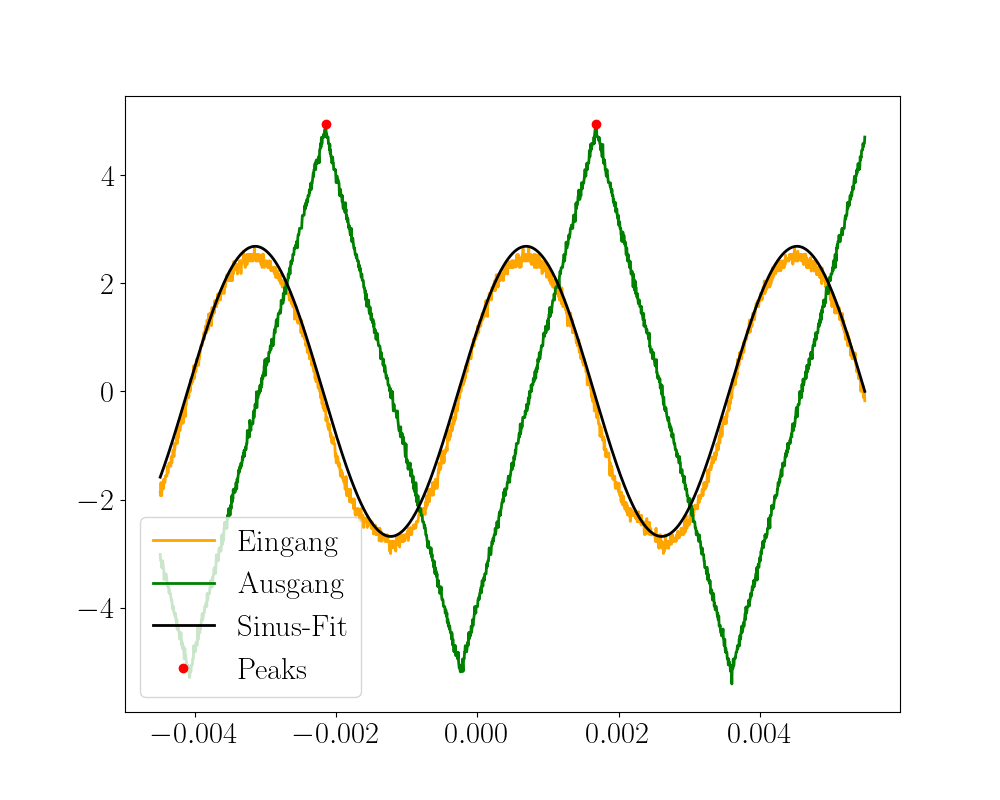
\includegraphics[width=0.8\textwidth]{../Ressourcen/signal_3.png}
  \caption{Ein- und Ausgangssignale des Generators, inklusive eines Sinus-Fits und gekennzeichneter Maxima.}
  \label{fig:10}
\end{figure}
Es lassen sich die relevanten Frequenzen $f$ und Amplituden $A$ der Signale bestimmen, welche in \autoref{tab:4} aufgeführt sind.
\begin{table}[H]
  \centering
  \caption{Charakteristische Signalparameter}
  \begin{tabular}{c | c c}
  \toprule
   Signal & $f\mathbin{/}\unit{\hertz}$ & $A\mathbin{/}\unit{\volt}$\\
  \midrule
  Eingang & 260.33 & 2.68\\
  Ausgang & 260.42 & 4.94\\
  \bottomrule
  \end{tabular}
  \label{tab:4}
\end{table}
Mittels \autoref{eqn:fdrei} lässt sich die theoretische Frequenz als 
\begin{align}
  f_\text{theorie} = \SI{2500}{\hertz}
\end{align}
und die theoretische Ausgangsamplitude mit \autoref{eqn:amp2} zu
\begin{align}
  A_\text{theorie} = \SI{31.4}{\volt}
\end{align}
berechnen.
\subsection{Generator mit variierender Amplitude}
Wie bereits in \autoref{subsec:vargen} beschrieben, tritt beim Anlegen einer Rechteckspannung eine gedämpfte Oszillation auf. Die resultierenden vom Oszilloskop exportierten Daten sind in \autoref{fig:genvarAmp} dargestellt.
\begin{figure}[H]
  \centering
  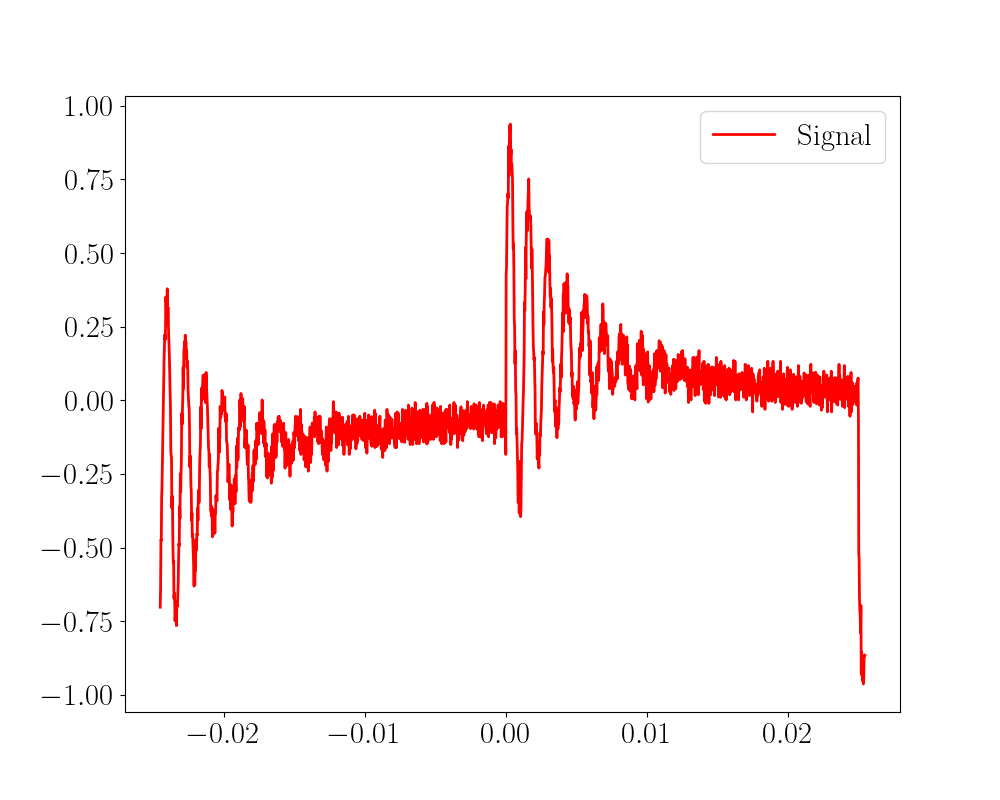
\includegraphics[width=0.8\textwidth]{Ressourcen/signal_13.png}
  \caption{Aufgenommenes Signal des Generators.}
  \label{fig:genvarAmp}
\end{figure}
Nachdem die Maxima der Ausgangsspannung identifiziert wurden, kann eine Exponentialfunktion an diese angepasst werden, wie in \autoref{fig:11} zu sehen.
\begin{figure}[H]
  \centering
  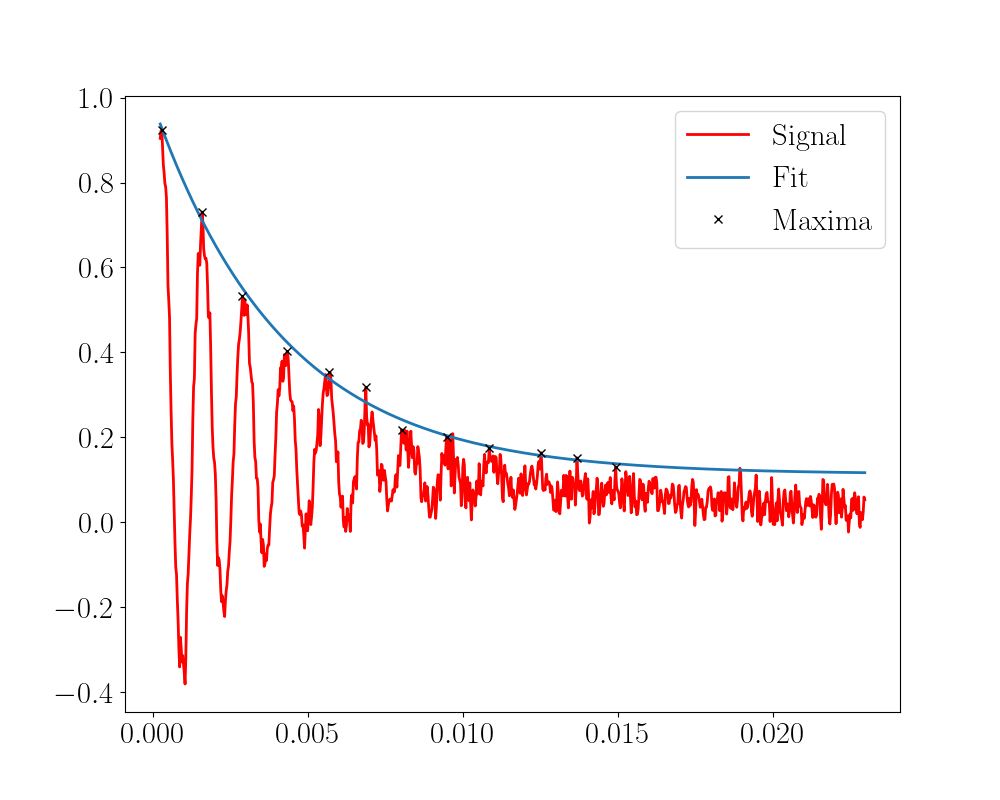
\includegraphics[width=0.8\textwidth]{Ressourcen/genvar_plot.png}
  \caption{Plot zur Bestimmung der Abklingzeit.}
  \label{fig:11}
\end{figure}

Für die gefundene Ausgleichsfunktion, welche der Form $f(x) = A \cdot \exp\left(-\frac{t}{\tau}\right) + b$ mit dem zusätzlichen Korrekturparameter $b$ entspricht, ergeben sich die folgenden Parameter:


\begin{align*}
    A &= (0.875 \pm 0.02)\,\unit{\volt} \;,\\
    \tau &= (4.19 \pm 0.27)\,\unit{\milli\second} \;,\\
    b &= (0.113 \pm 0.015)\,\unit{\volt} \;.
\end{align*}

Der Parameter $\tau$ beschreibt eben die gesuchte Abklingzeit der Schaltung.\\
\\
Theoretisch lässt sich die Abklingzeit gemäß \autoref{eqn:tau} zu $\tau_\text{theorie} = 4.4\,\unit{\milli\second}$ bestimmen, wobei als Dämpfungsfaktor $\eta = 1$ angenommen wurde.

\section{Diskussion}\label{sec:diskussion}

In dieser Diskussion werden die berechneten Werte der Experimente den theoretischen Werten gegenübergestellt, um die Genauigkeit und Zuverlässigkeit der Ergebnisse zu bewerten.

\begin{table}[H]
  \centering
  \caption{Vergleich der berechneten und theoretischen Werte für den invertierenden Verstärker}
  \begin{tabular}{c | c c | c}
  \toprule
  Parameter & Berechnet & Theoretisch & Abweichung \\
  \midrule
  Verstärkung $V$ & $91.70 \pm 4.82$ & 100 & $(8.29\pm4.82)$\%\\
  Grenzfrequenz $f_\text{grenz}$ (Hz) & $9538.98 \pm 962.41$ & - & - \\
  \bottomrule
  \end{tabular}
  \label{tab:inv_verstarker}
\end{table}

Die Abweichung der Verstärkung ist grundsätzlich Akzeptabel.

\begin{table}[H]
  \centering
  \caption{Vergleich der berechneten und theoretischen Werte für den Integrator}
  \begin{tabular}{c | c c | c}
  \toprule
  Parameter & Berechnet & Theoretisch & Abweichung \\
  \midrule
  Steigung $m$ & $-0.902 \pm 0.013$ & $-1$ & $(9.79\pm1.3)$\%\\
  Achsenabschnitt $b$ & $4.62 \pm 0.05$ & $6.91$ & $(33.1\pm0.7)$\%\\
  \bottomrule
  \end{tabular}
  \label{tab:integrator}
\end{table}

Diese Abweichungen könnten wie bei dem invertierenden Verstärker durch Messungenauigkeiten oder Nicht-Idealitäten im Schaltungsaufbau verursacht worden sein.

\begin{table}[H]
  \centering
  \caption{Vergleich der berechneten und theoretischen Werte für den Differentiator}
  \begin{tabular}{c | c c | c}
  \toprule
  Parameter & Berechnet & Theoretisch & Abweichung \\
  \midrule
  Steigung & $0.949 \pm 0.008$ & $1$ & $(5.1\pm0.8)$\%\\
  Achsenabschnitt & $-4.07 \pm 0.05$ & $-6.11$ & $(33.1\pm0.7)$\%\\
  \bottomrule
  \end{tabular}
  \label{tab:differentiator}
\end{table}

Auch hier könnten Nicht-Idealitäten der verwendeten Bauteile oder Messungenauigkeiten eine Rolle spielen, da das Oszillatorsignal über den gesamten Experimentalzeitrum nicht zuverlässig war.

\begin{table}[H]
  \centering
  \caption{Vergleich der berechneten und theoretischen Werte für den Schmitt-Trigger}
  \begin{tabular}{c | c c | c}
  \toprule
  Parameter & Berechnet & Theoretisch & Abweichung \\
  \midrule
  Schwellenwert (V) & $3.112$ & $3.2$ & $2.75\%$\\
  \bottomrule
  \end{tabular}
  \label{tab:schmitt_trigger}
\end{table}

\begin{table}[H]
  \centering
  \caption{Vergleich der berechneten und theoretischen Werte für den Generator}
  \begin{tabular}{c | c c | c}
  \toprule
  Parameter & Berechnet & Theoretisch & Abweichung \\
  \midrule
  Frequenz (Hz) & $260.42$ & $2500$ & $89.6$\%\\
  Amplitude (V) & $4.94$ & $31.4$ & $83.2$\%\\
  \bottomrule
  \end{tabular}
  \label{tab:generator}
\end{table}

Die berechnete Frequenz und Amplitude des Generators weichen erheblich von den theoretischen Werten ab. Dies könnte auf systematische Fehler im Versuchsaufbau zurückzuführen sein, da für verschiedene Operationsverstärker verschiedene oder sogar keine Signale zu erkennen waren. Des weiteren kann erneut das Oszilloskop das Ergebnis verfälschen, da die korrekte Erfassung der Werte durch starke Fluktuationen und Instabilität des Signals erschwert wurde.

\begin{table}[H]
  \centering
  \caption{Vergleich der berechneten und theoretischen Werte für den Generator mit variierender Amplitude}
  \begin{tabular}{c | c c | c}
  \toprule
  Parameter & Berechnet & Theoretisch & Abweichung \\
  \midrule
  Abklingzeit (ms) & $4.19 \pm 0.27$ & $4.4$ & $(5.01)\%$\\
  \bottomrule
  \end{tabular}
  \label{tab:gen_var_amp}
\end{table}

Die berechnete Abklingzeit liegt bei $4.19 \pm 0.27\, \mathrm{ms}$, was einer Abweichung von $-4.8\%$ vom theoretischen Wert entspricht. Diese geringe Abweichung deutet auf eine hohe Genauigkeit der Messung hin.

Die Proportionalitätstendenzen für Integrator und Differentiator decken sich mit der Erwartung, ebenso ähnelt der Abklingprozess stark der Lösung der zugehörigen DGL.


\section{Literaturverzeichnis}\label{sec:literaturverzeichnis}
\printbibliography[heading = none]
\newpage

\section{Anhang}\label{sec:anhang}

\end{document}
